\chapter{Cromatina y epigenética}\label{ch:b3:chromatin-epigenetics}

Dos ratones de la misma camada, genéticamente idénticos hasta la última
base, se sientan uno al lado del otro: uno es delgado y pardo, el otro
gordo y amarillo, y acabará siendo diabético. Una gata carey lleva
manchas naranjas y negras aunque todas las células de su piel llevan los
mismos dos cromosomas X. Un niño hereda la misma pérdida de un trozo del
cromosoma 15 que otro niño, y uno tiene el síndrome de Prader--Willi y el
otro el de Angelman --- la única diferencia es de qué progenitor venía la
deleción. Nada de esto está escrito en la secuencia del ADN. Está escrito
\emph{sobre} ella: en la manera en que dos metros de ADN se empaquetan en
un núcleo de diez micrómetros, en los pequeños grupos químicos unidos a
las proteínas de empaquetamiento y a las propias citosinas, y en la
maquinaria que copia esas marcas de una célula a sus hijas. Este capítulo
trata de esa segunda capa de información, de sus portadores moleculares y
de los límites honrados de lo que puede recordar.

\section{La cromatina: el ADN sobre un carrete}

\begin{definition}[Nucleosoma y cromatina]\label{def:b3:chromatin-epigenetics:nucleosome}
\index{nucleosoma}\index{cromatina}\index{histona}\index{eucromatina}\index{heterocromatina}
La \emph{cromatina} es el complejo del ADN con proteínas en el que existe
el genoma dentro de un núcleo eucariota. Su unidad repetida es el
\emph{nucleosoma}: \qty{147}{bp} de ADN enrollados en $1.65$ vueltas
levógiras alrededor de un octámero de \emph{histonas} --- dos copias de
cada una de las proteínas pequeñas y muy básicas H2A, H2B, H3 y H4 ---,
seguidos de un \emph{enlazador} de \qtyrange{20}{60}{bp} hasta el
nucleosoma siguiente. Una quinta histona, H1, se une al enlazador donde
entra y sale del núcleo de la partícula y ayuda a que las cuentas se
apilen unas contra otras. Cada histona del núcleo lleva una \emph{cola}
amino-terminal desestructurada de unos \numrange{20}{40} residuos que
sobresale de la partícula. La cromatina que se tiñe débilmente, está poco
condensada y se transcribe es la \emph{eucromatina}; la cromatina densa,
de replicación tardía y en gran parte silenciosa, en los centrómeros, los
telómeros y las secuencias repetidas, es la \emph{heterocromatina}.
\end{definition}

\begin{proof}[Evidencia]
Hewish y Burgoyne (1973) digirieron núcleos de hígado de rata con una
nucleasa endógena y encontraron que el ADN no salía como una mancha
continua sino como una escalera de fragmentos cuyas longitudes eran
múltiplos de unos \qty{200}{bp}: el ADN estaba protegido a intervalos
regulares y solo se cortaba entre ellos. Kornberg (1974) demostró que la
unidad protegida era una partícula de ocho \omterm{def:b3:chromatin-epigenetics:nucleosome}{histonas} con unos
\qty{200}{bp}, y las micrografías electrónicas de \omterm{def:b3:chromatin-epigenetics:nucleosome}{cromatina} extendida con
suavidad mostraron las ``cuentas de un collar''. Luger y colaboradores
(1997) resolvieron la estructura cristalina de la partícula nuclear a
\qty{2.8}{\angstrom}: \qty{147}{bp} y un octámero con las colas saliendo
entre las vueltas del ADN.
\end{proof}

\begin{omfigure}
\begin{tikzpicture}[every node/.style={font=\scriptsize}, >=stealth]
  % beads on a string
  \foreach \x/\y in {0/0, 2.2/0.5, 4.4/0, 6.6/0.5, 8.8/0} {
    \fill[omDef!30] (\x,\y) circle (0.42);
    \draw[very thick, omThm!70!black] (\x,\y) circle (0.5);
  }
  \draw[very thick, omThm!70!black] (-1.1,-0.1) -- (0-0.47,-0.17);
  \draw[very thick, omThm!70!black] (0.47,-0.17) -- (2.2-0.47,0.33);
  \draw[very thick, omThm!70!black] (2.67,0.33) -- (4.4-0.47,-0.17);
  \draw[very thick, omThm!70!black] (4.87,-0.17) -- (6.6-0.47,0.33);
  \draw[very thick, omThm!70!black] (7.07,0.33) -- (8.8-0.47,-0.17);
  \draw[very thick, omThm!70!black] (9.27,-0.17) -- (10.4,-0.1);
  % tails
  \foreach \x/\y in {0/0, 4.4/0, 8.8/0} { \draw[omProp, thick] (\x,\y+0.5) .. controls (\x-0.2,\y+0.9) .. (\x+0.1,\y+1.15); \draw[omProp, thick] (\x,\y-0.5) .. controls (\x+0.2,\y-0.9) .. (\x-0.1,\y-1.15); }
  \foreach \x/\y in {2.2/0.5, 6.6/0.5} { \draw[omProp, thick] (\x,\y+0.5) .. controls (\x-0.2,\y+0.9) .. (\x+0.1,\y+1.15); }
  % H1
  \fill[omMeth!70!black] (1.55,0.05) circle (0.12); \fill[omMeth!70!black] (5.95,0.05) circle (0.12);
  % labels
  \node[above, align=center] at (2.2,1.75) {colas de histona\\(acetilación, metilación)};
  \node[below, align=center] at (4.4,-1.35) {partícula nuclear: octámero\\$+$ \qty{147}{bp}, $1.65$ vueltas};
  \node[below, align=center] at (7.7,-0.55) {ADN enlazador\\\qtyrange{20}{60}{bp}};
  \node[below] at (5.95,-0.1) {H1};
  \draw[<->] (-0.5,-2.2) -- (2.2-0.5,-2.2) node[midway, below] {repetición $\approx \qty{200}{bp}$, \qty{11}{nm}};
  \draw[gray] (-0.5,-1.95) -- (-0.5,-2.35); \draw[gray] (1.7,-1.95) -- (1.7,-2.35);
\end{tikzpicture}

{\small La fibra de \qty{10}{nm}: núcleos de \omterm{def:b3:chromatin-epigenetics:nucleosome}{nucleosoma} (azul) sobre un
ADN continuo (rojo), cada cuenta un octámero de \omterm{def:b3:chromatin-epigenetics:nucleosome}{histonas} con sus colas
(naranja) hacia fuera, y la \omterm{def:b3:chromatin-epigenetics:nucleosome}{histona} enlazadora H1 (verde) en el punto de
entrada y salida. Unos seis \omterm{def:b3:chromatin-epigenetics:nucleosome}{nucleosomas} ocupan la longitud que tendrían
\qty{1200}{bp} de ADN desnudo.}
\end{omfigure}

\begin{omfigure}
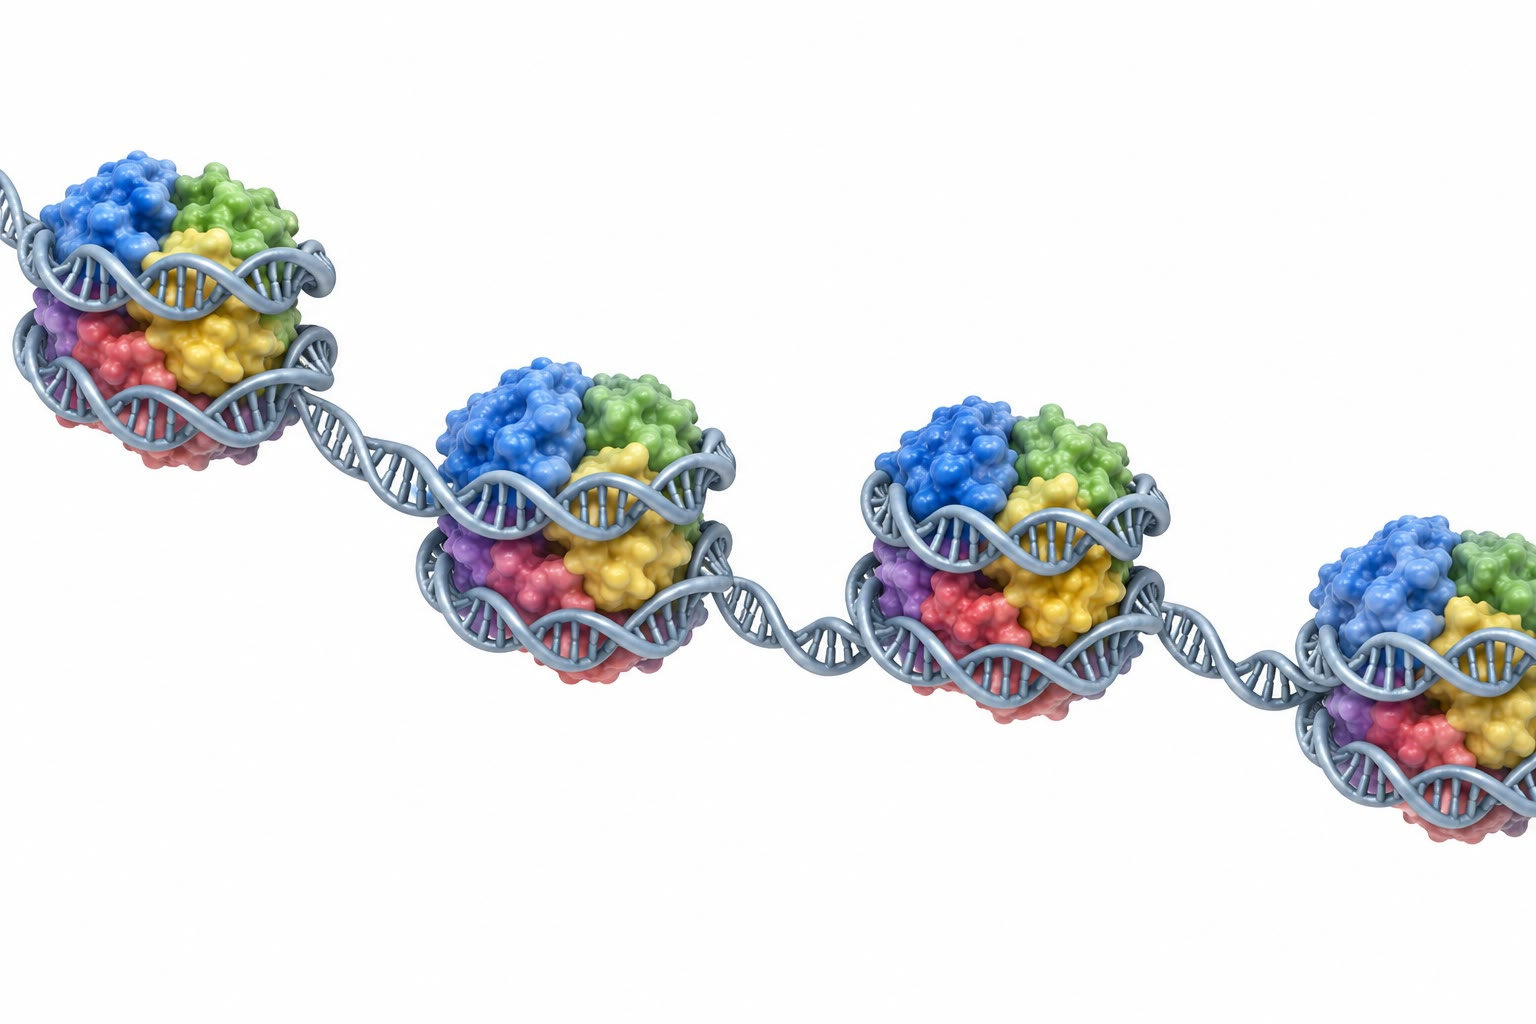
\includegraphics[width=0.6\linewidth]{images/book5/ai/b5-01-nucleosomes.jpg}

{\small La \omterm{def:b3:chromatin-epigenetics:nucleosome}{cromatina} a escala molecular: la doble hélice enrollada sobre
núcleos de \omterm{def:b3:chromatin-epigenetics:nucleosome}{histonas} sucesivos, las ``cuentas de un collar'' que reveló la
escalera de la nucleasa.}
\end{omfigure}

\begin{proposition}[Niveles de condensación]\label{prop:b3:chromatin-epigenetics:compaction}
\index{razón de empaquetamiento}\index{bucle de cromatina}\index{dominio de asociación topológica}
La \emph{\omterm{prop:b3:chromatin-epigenetics:compaction}{razón de empaquetamiento}} de una estructura de \omterm{def:b3:chromatin-epigenetics:nucleosome}{cromatina} es la
longitud del ADN que contiene dividida por la longitud de la estructura.
El enrollamiento en la fibra de \qty{10}{nm} da una razón de unos $6$:
los \qty{68}{nm} de una repetición de \qty{200}{bp} se comprimen en una
sola cuenta de \qty{11}{nm}. En el núcleo en interfase la fibra no se
enrolla en otra fibra regular más gruesa, como la dibujaron los libros de
texto durante mucho tiempo, sino que se pliega en \emph{bucles} de
decenas a centenares de kilobases sujetos por su base por complejos de
cohesina en forma de anillo y por la proteína CTCF, que se une al ADN;
los bucles se agrupan en \emph{\omterm{prop:b3:chromatin-epigenetics:compaction}{dominios de asociación topológica}} (TAD)
de aproximadamente una megabase, dentro de los cuales un gen se encuentra
con sus reguladores mucho más a menudo que con nada de fuera. Un
cromosoma mitótico, el estado más condensado, tiene una \omterm{prop:b3:chromatin-epigenetics:compaction}{razón de
empaquetamiento} cercana a \num{10000}: los \qty{4}{cm} de ADN de un
cromosoma humano medio se pliegan en un bastón de \qty{4}{\micro m}.
\end{proposition}

\begin{example}[Dos metros en diez micrómetros]\label{ex:b3:chromatin-epigenetics:two-metres}
Un núcleo humano diploide contiene $6.4\times 10^{9}$ pares de bases. A
\qty{0.34}{nm} por par de bases eso son \qty{2.2}{m} de doble hélice, en
un núcleo de unos \qty{10}{\micro m} de diámetro. Se empaquetan en
$6.4\times 10^{9}/200 \approx 3.2\times 10^{7}$ \omterm{def:b3:chromatin-epigenetics:nucleosome}{nucleosomas}, cada uno con
unos \qty{108}{kDa} de \omterm{def:b3:chromatin-epigenetics:nucleosome}{histona} frente a \qty{96}{kDa} de ADN
(\qty{147}{bp} a \qty{650}{Da} por par): el núcleo contiene
aproximadamente tanta \omterm{def:b3:chromatin-epigenetics:nucleosome}{histona} como ADN en masa. El propio ADN, tratado
como un cilindro de \qty{2}{nm} de diámetro, ocupa un volumen de solo
unos \qty{7}{\micro m^3}, un \qty{1}{\%} de un núcleo esférico de radio
\qty{5}{\micro m}; el problema del empaquetamiento es de enredo y de
acceso, no de espacio.
\end{example}

\section{El código de histonas}

\begin{definition}[Modificaciones de las histonas]\label{def:b3:chromatin-epigenetics:histone-code}
\index{código de histonas}\index{acetilación}\index{metilación de histonas}\index{escritor}\index{lector}\index{borrador}
Los residuos de las colas de las \omterm{def:b3:chromatin-epigenetics:nucleosome}{histonas} se modifican covalentemente:
\emph{acetilación} de las lisinas (que neutraliza su carga positiva y
afloja la sujeción del ADN), \emph{metilación} de lisinas y argininas
(uno, dos o tres grupos metilo, sin cambio de carga), fosforilación de
serinas, ubiquitinación de lisinas. Una modificación se nombra por
\omterm{def:b3:chromatin-epigenetics:nucleosome}{histona}, residuo y grupo: H3K4me3 es la \omterm{def:b3:chromatin-epigenetics:nucleosome}{histona} H3, lisina 4,
trimetilada; H3K27ac es la H3 con la lisina 27 acetilada. El \emph{código
de \omterm{def:b3:chromatin-epigenetics:nucleosome}{histonas}} es la correlación entre las combinaciones de marcas y el
estado del gen subyacente: H3K4me3 y H3K27ac en los promotores y los
potenciadores activos, H3K36me3 a lo largo de los cuerpos de los genes
transcritos, H3K9me3 en la \omterm{def:b3:chromatin-epigenetics:nucleosome}{heterocromatina} constitutiva, H3K27me3 en los
genes silenciados durante el desarrollo. Las enzimas que añaden una marca
son \emph{escritores} (histona-acetiltransferasas, HAT;
metiltransferasas), las que la quitan son \emph{borradores}
(histona-desacetilasas, HDAC; desmetilasas), y las proteínas que se unen
a una marca y actúan a partir de ella son \emph{lectores}: un
\emph{bromodominio} une acetil-lisina, y un \emph{cromodominio},
metil-lisina.
\end{definition}

\begin{proposition}[Las marcas se leen, no solo se sienten]\label{prop:b3:chromatin-epigenetics:readers}
\index{HP1}\index{Polycomb}\index{PRC2}\index{Trithorax}
La \omterm{def:b3:chromatin-epigenetics:histone-code}{acetilación} actúa en parte por electrostática --- una cola acetilada
sujeta su ADN con menos fuerza y la fibra se abre ---, pero la mayoría de
las marcas actúan reclutando \omterm{def:b3:chromatin-epigenetics:histone-code}{lectores}. La H3K9me3 la une el cromodominio
de la \emph{proteína de \omterm{def:b3:chromatin-epigenetics:nucleosome}{heterocromatina} HP1}, que dimeriza, tiende un
puente entre \omterm{def:b3:chromatin-epigenetics:nucleosome}{nucleosomas} vecinos y recluta a la mismísima
metiltransferasa (SUV39H) que escribe H3K9me3 en el \omterm{def:b3:chromatin-epigenetics:nucleosome}{nucleosoma} siguiente:
la marca se propaga a lo largo de la fibra hasta encontrar un límite y
condensa lo que cubre. La H3K27me3 la escribe el \emph{complejo represivo
Polycomb 2} (PRC2, subunidad catalítica EZH2), la lee PRC1, que
ubiquitina la H2A y condensa la fibra, y el complejo es a su vez
estimulado por la marca que produce; el grupo de proteínas
\emph{Trithorax} escribe la marca opuesta, H3K4me3, y mantiene activos
los genes del desarrollo propios de un tipo celular dado. Cada uno de
estos bucles --- un \omterm{def:b3:chromatin-epigenetics:histone-code}{lector} que recluta a un \omterm{def:b3:chromatin-epigenetics:histone-code}{escritor} --- es una
retroalimentación positiva que permite a un estado mantenerse una vez
establecido, que es lo que necesita una marca heredable.
\end{proposition}

\begin{omfigure}
\begin{tikzpicture}[every node/.style={font=\scriptsize}, >=stealth]
  % nucleosomes with tails
  \foreach \x in {0,2,4,6} { \draw[thick, omDef, fill=omDef!20] (\x,0) circle (0.45); \draw[omProp, thick] (\x,0.45) -- (\x,1.15); }
  % marks
  \fill[omThm] (2,1.15) circle (0.11); \fill[omThm] (4,1.15) circle (0.11);
  \fill[omMeth!80!black] (0,1.15) circle (0.11);
  \node[left] at (-0.5,1.15) {ac};
  \node[right, align=left] at (6.15,1.15) {me3};
  % HP1 reader
  \draw[thick, fill=omExo!30] (2.6,1.7) ellipse (0.5 and 0.25); \node at (2.6,1.7) {lector};
  \draw[thick, fill=omExo!30] (4.2,2.35) ellipse (0.55 and 0.25); \node at (4.2,2.35) {escritor};
  \draw[->, thick] (2.9,1.9) -- (3.75,2.2);
  \draw[->, thick, omThm] (4.6,2.15) .. controls (5.6,2.0) and (6.1,1.8) .. (6.05,1.3);
  \node[right, align=left, font=\scriptsize] at (6.6,2.0) {se propaga al\\nucleosoma siguiente};
  \draw[->, thick, gray] (2.2,1.3) -- (2.45,1.5);
  % eraser
  \draw[thick, fill=omExo!30] (0.6,2.2) ellipse (0.5 and 0.25); \node at (0.6,2.2) {borrador};
  \draw[->, thick, omMeth!80!black] (0.3,2.0) -- (0.05,1.35);
  % DNA
  \draw[very thick, omThm!70!black] (-0.9,-0.3) -- (-0.45,-0.05) (0.45,-0.05) -- (1.55,-0.05) (2.45,-0.05) -- (3.55,-0.05) (4.45,-0.05) -- (5.55,-0.05) (6.45,-0.05) -- (7.2,-0.3);
  \node[below, align=center] at (0,-0.6) {abierta: el grupo acetilo\\quita una carga};
  \node[below, align=center] at (5,-0.6) {cerrada: HP1 lee H3K9me3\\y recluta la metilasa de K9};
\end{tikzpicture}

{\small La lógica escritor--lector--borrador. Un \omterm{def:b3:chromatin-epigenetics:histone-code}{lector} unido a una marca
en un \omterm{def:b3:chromatin-epigenetics:nucleosome}{nucleosoma} recluta al \omterm{def:b3:chromatin-epigenetics:histone-code}{escritor} que pone la misma marca en el
siguiente, de modo que el estado se propaga y se copia a sí mismo; los
\omterm{def:b3:chromatin-epigenetics:histone-code}{borradores} se oponen. Los grupos acetilo (verde) abren la fibra; la
H3K9me3 (rojo) la cierra.}
\end{omfigure}

\begin{method}[Inmunoprecipitación de cromatina (ChIP)]\label{met:b3:chromatin-epigenetics:chip}
\index{ChIP}\index{inmunoprecipitación de cromatina}
Para cartografiar dónde se sitúa una marca o una proteína en el genoma:
(1) se entrecruzan las proteínas con el ADN en células vivas con
formaldehído; (2) se fragmenta la \omterm{def:b3:chromatin-epigenetics:nucleosome}{cromatina} en trozos de unos pocos
centenares de pares de bases; (3) se precipitan los fragmentos con un
anticuerpo contra la marca (por ejemplo H3K27me3) unido a bolas; (4) se
revierten los entrecruzamientos y se purifica el ADN; (5) se secuencia
(ChIP-seq) y se cuentan las lecturas a lo largo del genoma: los picos son
los lugares donde estaba la marca. Un control de ADN de partida sin
anticuerpo fija el fondo. La resolución es la de los fragmentos, de
aproximadamente un \omterm{def:b3:chromatin-epigenetics:nucleosome}{nucleosoma}.
\end{method}

\begin{remark}[Código o correlación]\label{rem:b3:chromatin-epigenetics:code}
La palabra ``código'' exagera. Muchas marcas son consecuencia de la
transcripción más que causa suya (la H3K36me3 la deposita una
metiltransferasa que viaja con la polimerasa), y quitar un \omterm{def:b3:chromatin-epigenetics:histone-code}{escritor}
cambia la expresión mucho menos de lo que sugiere la distribución de la
marca. Lo que sí está bien establecido es que unas pocas marcas ---
H3K9me3, H3K27me3 y la \omterm{def:b3:chromatin-epigenetics:methylation}{metilación del ADN} que sigue --- llevan un
silenciamiento que se propaga solo y sobrevive a la señal que lo inició.
\end{remark}

\section{La metilación del ADN y la copia de una marca}

\begin{definition}[Metilación del ADN]\label{def:b3:chromatin-epigenetics:methylation}
\index{metilación del ADN}\index{CpG}\index{isla CpG}\index{DNMT1}\index{metilación de mantenimiento}\index{metilación de novo}
En los vertebrados se añade un grupo metilo al carbono 5 de la citosina
casi solo en el dinucleótido \emph{CpG} (una C seguida de una G en la
misma hebra), una secuencia que es su propio complemento, de modo que un
CpG metilado suele estarlo en ambas hebras. Entre el
\qtyrange{70}{80}{\%} de los CpG de una célula humana están metilados, y
los promotores metilados están silenciosos: los grupos metilo los leen
proteínas de unión a CpG metilado (MeCP2, MBD1--4) que reclutan HDAC y
metilasas de H3K9, y además bloquean directamente a varios factores de
transcripción. La excepción son las \emph{islas CpG}, tramos de alrededor
de una kilobase, ricos en G y C y en CpG, que se sitúan en los promotores
de la mayoría de los genes constitutivos y permanecen sin metilar en las
células normales. El grupo metilo lo escriben las
\emph{ADN-metiltransferasas}: DNMT3A y DNMT3B llevan a cabo la
\emph{metilación de novo} de los sitios no metilados, y \emph{DNMT1}, que
prefiere un CpG hemimetilado --- una hebra metilada y la otra no ---,
realiza la \emph{metilación de mantenimiento} detrás de la horquilla de
replicación. La eliminación es pasiva, por replicación sin mantenimiento,
o activa, por las enzimas TET, que oxidan la 5-metilcitosina a
5-hidroximetilcitosina y más allá hasta que la reparación por escisión de
bases la sustituye por una citosina normal.
\end{definition}

\begin{example}[Por qué el genoma es pobre en CpG]\label{ex:b3:chromatin-epigenetics:cpg-deficit}
El genoma humano tiene un \qty{42}{\%} de G$+$C, de modo que si las bases
fueran independientes un \omterm{def:b3:chromatin-epigenetics:methylation}{CpG} aparecería con una frecuencia de
$0.21\times 0.21 \approx 0.044$, unas $2.8\times 10^{8}$ veces en el
genoma diploide. El
número observado es de unos $5.6\times 10^{7}$, la quinta parte. La razón
es la propia marca: una citosina metilada que pierde su grupo amino se
convierte en timina, una base normal que la reparación no puede
reconocer como errónea, mientras que una citosina sin metilar se desamina
a uracilo, que sí se escinde. A lo largo del tiempo evolutivo los \omterm{def:b3:chromatin-epigenetics:methylation}{CpG}
metilados han mutado a TpG y CpA, y solo las islas sin metilar han
conservado sus \omterm{def:b3:chromatin-epigenetics:methylation}{CpG}. La marca ha dejado su firma en la secuencia.
\end{example}

\begin{theorem}[Mantenimiento de un estado de metilación a lo largo de las divisiones]\label{thm:b3:chromatin-epigenetics:maintenance}
\index{memoria epigenética}\index{cadena de Markov!metilación}
Considérese un solo sitio \omterm{def:b3:chromatin-epigenetics:methylation}{CpG}, seguido a lo largo de un linaje de
células. En cada división la citosina de la hebra nueva se metila con
probabilidad $\mu$ si la citosina de la hebra molde está metilada
(eficiencia de mantenimiento) y con probabilidad $\delta$ si no lo está
(tasa de novo). Sea $p_{n}$ la probabilidad de que el sitio esté metilado
después de $n$ divisiones. Entonces
\[
p_{n+1} = \mu\, p_{n} + \delta\,(1 - p_{n}),
\qquad
p_{n} = p^{*} + (p_{0} - p^{*})\,(\mu - \delta)^{n},
\qquad
p^{*} = \frac{\delta}{1 - \mu + \delta}.
\]
Todo sitio deriva hacia el mismo equilibrio $p^{*}$, sea cual sea su
estado de partida, y la memoria del estado inicial decae
geométricamente con razón $\mu - \delta$. Una marca se recuerda durante
unas $1/(1 - \mu + \delta)$ divisiones; la memoria fiel de una
\emph{diferencia} entre sitios exige por tanto un $\mu$ muy próximo a $1$
y un $\delta$ muy próximo a $0$, o bien una retroalimentación que haga
depender $\mu$ y $\delta$ del estado del vecindario.
\end{theorem}
\begin{proof}
La recurrencia es la ley de la probabilidad total sobre los dos estados
de la hebra molde. Su punto fijo resuelve $p^{*} = \mu p^{*} + \delta(1 -
p^{*})$, lo que da $p^{*}(1 - \mu + \delta) = \delta$. Restando la
ecuación del punto fijo de la recurrencia, $p_{n+1} - p^{*} = (\mu -
\delta)(p_{n} - p^{*})$, que iterado da la forma cerrada. Como
$0 \le \delta \le \mu \le 1$, la razón $\mu - \delta$ está en $[0,1]$ y
la desviación se encoge; se reduce a la mitad cada $\ln 2 / (-\ln(\mu -
\delta)) \approx \ln 2/(1 - \mu + \delta)$ divisiones cuando $\mu -
\delta$ está cerca de $1$.
\end{proof}

\begin{example}[Números]\label{ex:b3:chromatin-epigenetics:maintenance-numbers}
Los valores medidos en células de mamífero son $\mu \approx 0.99$ y
$\delta \approx 0.02$ por división en un \omterm{def:b3:chromatin-epigenetics:methylation}{CpG} típico. Entonces $p^{*} =
0.02/0.03 \approx 0.67$, próximo a la fracción metilada de todo el
genoma, y $\mu - \delta = 0.97$: un sitio completamente metilado dejado a
solas con la maquinaria estaría a medio camino de la media tras $\ln 2 /
0.03 \approx 23$ divisiones. Un promotor silenciado que siga
silencioso durante los centenares de divisiones de una vida necesita por
tanto algo más que la \omterm{def:b3:chromatin-epigenetics:methylation}{DNMT1}: los \omterm{def:b3:chromatin-epigenetics:histone-code}{lectores} de \omterm{def:b3:chromatin-epigenetics:methylation}{CpG} metilado reclutan
metilación de H3K9 y los \omterm{def:b3:chromatin-epigenetics:histone-code}{lectores} de H3K9 reclutan a DNMT3, de manera que
una isla densa de marcas eleva su propio $\mu$ hacia $1$ y baja el
$\delta$ de al lado hacia $0$. A la inversa, una célula que pierde la
\omterm{def:b3:chromatin-epigenetics:methylation}{DNMT1} pierde la marca de forma pasiva: con $\mu = \delta = 0$ la fracción
de hebras metiladas se reduce a la mitad en cada división.
\end{example}

\begin{omfigure}
\begin{tikzpicture}[every node/.style={font=\scriptsize}, >=stealth]
  % left: replication scheme
  \begin{scope}
    \draw[very thick, omThm!70!black] (0,1.2) -- (2.4,1.2); \draw[very thick, omThm!70!black] (0,0.9) -- (2.4,0.9);
    \foreach \x in {0.5,1.2,1.9} { \fill[omDef] (\x,1.2) circle (0.09); \fill[omDef] (\x,0.9) circle (0.09); }
    \node[above] at (1.2,1.3) {parental: ambas hebras metiladas};
    \draw[->, thick] (1.2,0.75) -- (1.2,0.15) node[midway, right] {replicación};
    \draw[very thick, omThm!70!black] (0,-0.1) -- (2.4,-0.1); \draw[very thick, gray] (0,-0.4) -- (2.4,-0.4);
    \foreach \x in {0.5,1.2,1.9} { \fill[omDef] (\x,-0.1) circle (0.09); \draw[omDef] (\x,-0.4) circle (0.09); }
    \node[left] at (-0.1,-0.25) {hemimetilado};
    \draw[->, thick] (1.2,-0.85) -- (1.2,-1.45) node[midway, right, align=left] {DNMT1, probabilidad $\mu$\\por sitio};
    \draw[very thick, omThm!70!black] (0,-1.7) -- (2.4,-1.7); \draw[very thick, gray] (0,-2.0) -- (2.4,-2.0);
    \foreach \x in {0.5,1.9} { \fill[omDef] (\x,-1.7) circle (0.09); \fill[omDef] (\x,-2.0) circle (0.09); }
    \fill[omDef] (1.2,-1.7) circle (0.09); \draw[omDef] (1.2,-2.0) circle (0.09);
    \node[below, align=center] at (1.2,-2.1) {restaurado, con un sitio omitido:\\la hebra nueva de la hija};
  \end{scope}
  % right: decay plot
  \begin{scope}[xshift=5.0cm, yshift=-2.3cm]
  \begin{axis}[
    width=6.6cm, height=4.6cm, axis lines=left,
    xmin=0, xmax=100, ymin=0, ymax=1.05,
    xlabel={divisiones $n$},
    xlabel style={font=\scriptsize, at={(axis description cs:0.5,-0.1)}, anchor=north},
    tick label style={font=\scriptsize}, xtick={0,25,50,75,100}, ytick={0,0.5,0.67,1},
    yticklabels={0,0.5,$p^{*}$,1}, clip=false,
  ]
  \addplot[very thick, omDef, domain=0:100, samples=60] {0.6667 + 0.3333*0.97^x};
  \addplot[very thick, omThm, domain=0:100, samples=60] {0.6667 - 0.6667*0.97^x};
  \addplot[dashed, gray, domain=0:100, samples=2] {0.6667};
  \addplot[thick, omMeth!80!black, domain=0:100, samples=60] {0.6667 + 0.3333*0.998^x};
  \node[font=\scriptsize] at (axis cs:-9,1.1) {$p_{n}$};
  \node[font=\scriptsize, omDef, anchor=south west] at (axis cs:45,0.82) {inicio metilado, $\mu = 0.99$};
  \node[font=\scriptsize, omThm, anchor=north west] at (axis cs:50,0.30) {inicio sin metilar};
  \node[font=\scriptsize, omMeth!80!black, anchor=south west] at (axis cs:30,1.02) {con retroalimentación, $\mu = 0.999$};
  \end{axis}
  \end{scope}
\end{tikzpicture}

{\small Izquierda: la \omterm{def:b3:chromatin-epigenetics:methylation}{metilación de mantenimiento}. Tras la replicación
todo \omterm{def:b3:chromatin-epigenetics:methylation}{CpG} queda hemimetilado; la \omterm{def:b3:chromatin-epigenetics:methylation}{DNMT1} copia la marca en la hebra nueva
con probabilidad $\mu$ por sitio. Derecha: el destino de un sitio a lo
largo de las divisiones para $\mu = 0.99$, $\delta = 0.02$ (en azul desde
metilado, en rojo desde sin metilar) --- ambos convergen en $p^{*} = 0.67$
--- y para un sitio cuya retroalimentación vecinal eleva $\mu$ a $0.999$
(verde).}
\end{omfigure}

\begin{method}[Leer la metilación: la secuenciación con bisulfito]\label{met:b3:chromatin-epigenetics:bisulfite}
\index{secuenciación con bisulfito}
La secuenciación por sí sola no ve un grupo metilo. Trátese el ADN
desnaturalizado con bisulfito de sodio: la citosina sin metilar se
desamina a uracilo, que se lee como T después de la PCR, mientras que la
5-metilcitosina queda protegida y sigue leyéndose como C. Secúnciese el
ADN convertido y compárese con la referencia: toda C que siga siendo C
estaba metilada, y toda C que se haya vuelto T no lo estaba. Hecho a
escala de todo el genoma (\omterm{met:b3:chromatin-epigenetics:bisulfite}{secuenciación con bisulfito} del genoma
completo), esto da el estado de metilación de cada uno de los
$2.8\times 10^{7}$ \omterm{def:b3:chromatin-epigenetics:methylation}{CpG} de un genoma haploide con resolución de una sola
base, como fracción de las células de la muestra.
\end{method}

\section{Inactivación del X e impronta genómica}

\begin{definition}[Inactivación del cromosoma X]\label{def:b3:chromatin-epigenetics:x-inactivation}
\index{inactivación del X}\index{corpúsculo de Barr}\index{Xist}\index{compensación de dosis}
En las hembras de mamífero uno de los dos cromosomas X de cada célula
somática se silencia transcripcionalmente al principio del desarrollo,
una forma de \emph{compensación de dosis} que iguala la expresión de los
genes ligados al X entre las hembras XX y los machos XY. El cromosoma
silenciado se condensa en un cuerpo denso pegado a la envoltura nuclear,
el \emph{corpúsculo de Barr}. La elección de qué X se silencia es
aleatoria en el embrión propiamente dicho y, una vez hecha, la heredan
clonalmente todas las descendientes de la célula. La inactivación la
inicia \emph{Xist}, un ARN no codificante de \qty{17}{kb} transcrito
desde el centro de inactivación del X del cromosoma que va a ser
silenciado: recubre ese cromosoma en cis, recluta a Polycomb (H3K27me3),
la variante de \omterm{def:b3:chromatin-epigenetics:nucleosome}{histona} macroH2A y finalmente la \omterm{def:b3:chromatin-epigenetics:methylation}{metilación del ADN} de los
promotores, y a partir de ahí el silencio se mantiene sin que haga falta
Xist en cada división. Alrededor del \qty{15}{\%} de los genes humanos
ligados al X escapan a la inactivación, en parte o del todo.
\end{definition}

\begin{proof}[Evidencia]
Barr y Bertram (1949) advirtieron un cuerpo denso en los núcleos de las
neuronas de gata pero no en las de gato. Ohno (1959) demostró que era un
cromosoma X entero, condensado. Lyon (1961) juntó las piezas: las ratonas
heterocigóticas para genes de color del pelaje ligados al X tienen un
pelaje en mosaico, con manchas que expresan un alelo o el otro, de modo
que cada mancha es un clon en el que un X, siempre el mismo, está
silencioso; lo mismo vale para las manchas naranjas y negras de una gata
carey, cuyo gen naranja está ligado al X, y para las glándulas sudoríparas
en mosaico de las mujeres portadoras de un alelo mutante de un gen ligado
al X. Un gato carey macho es casi siempre XXY.
\end{proof}

\begin{omfigure}
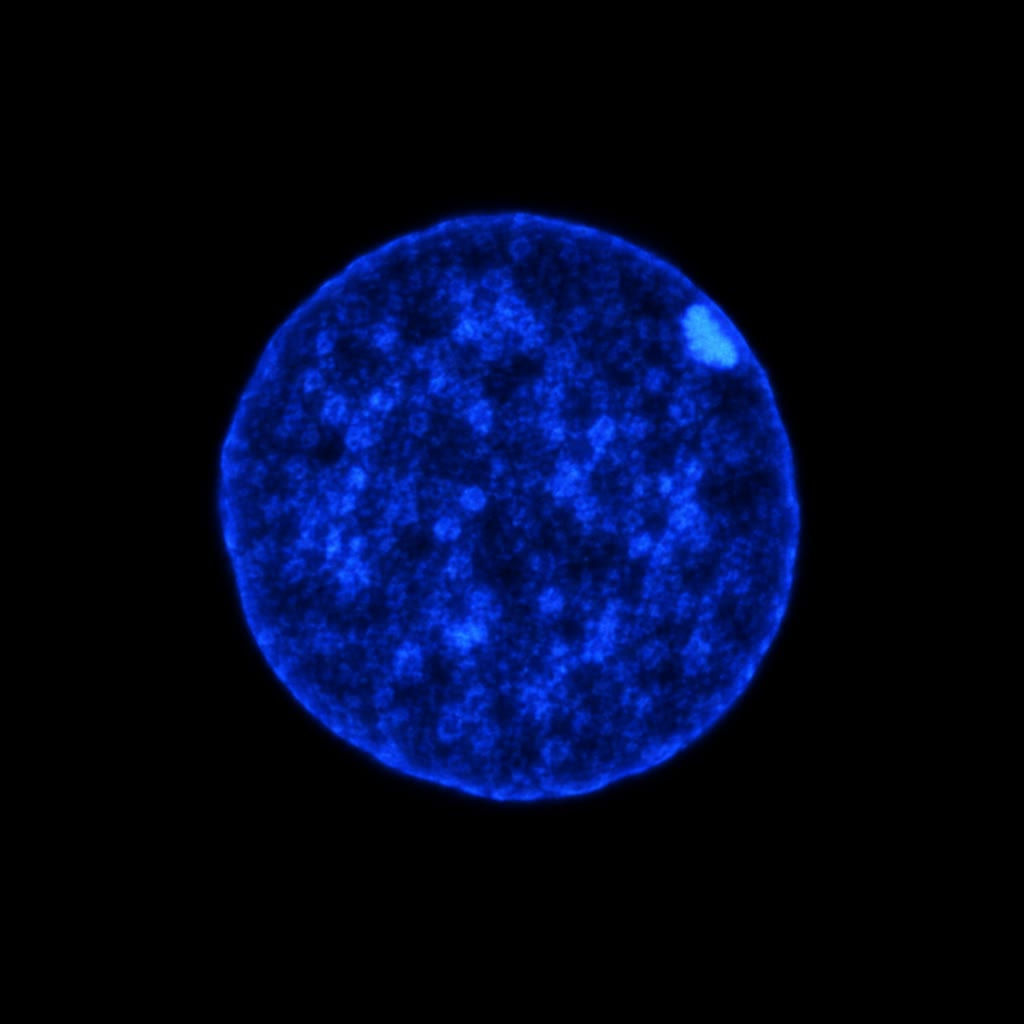
\includegraphics[width=0.42\linewidth]{images/book5/ai/b5-01-barr-body.jpg}\hspace{0.04\linewidth}
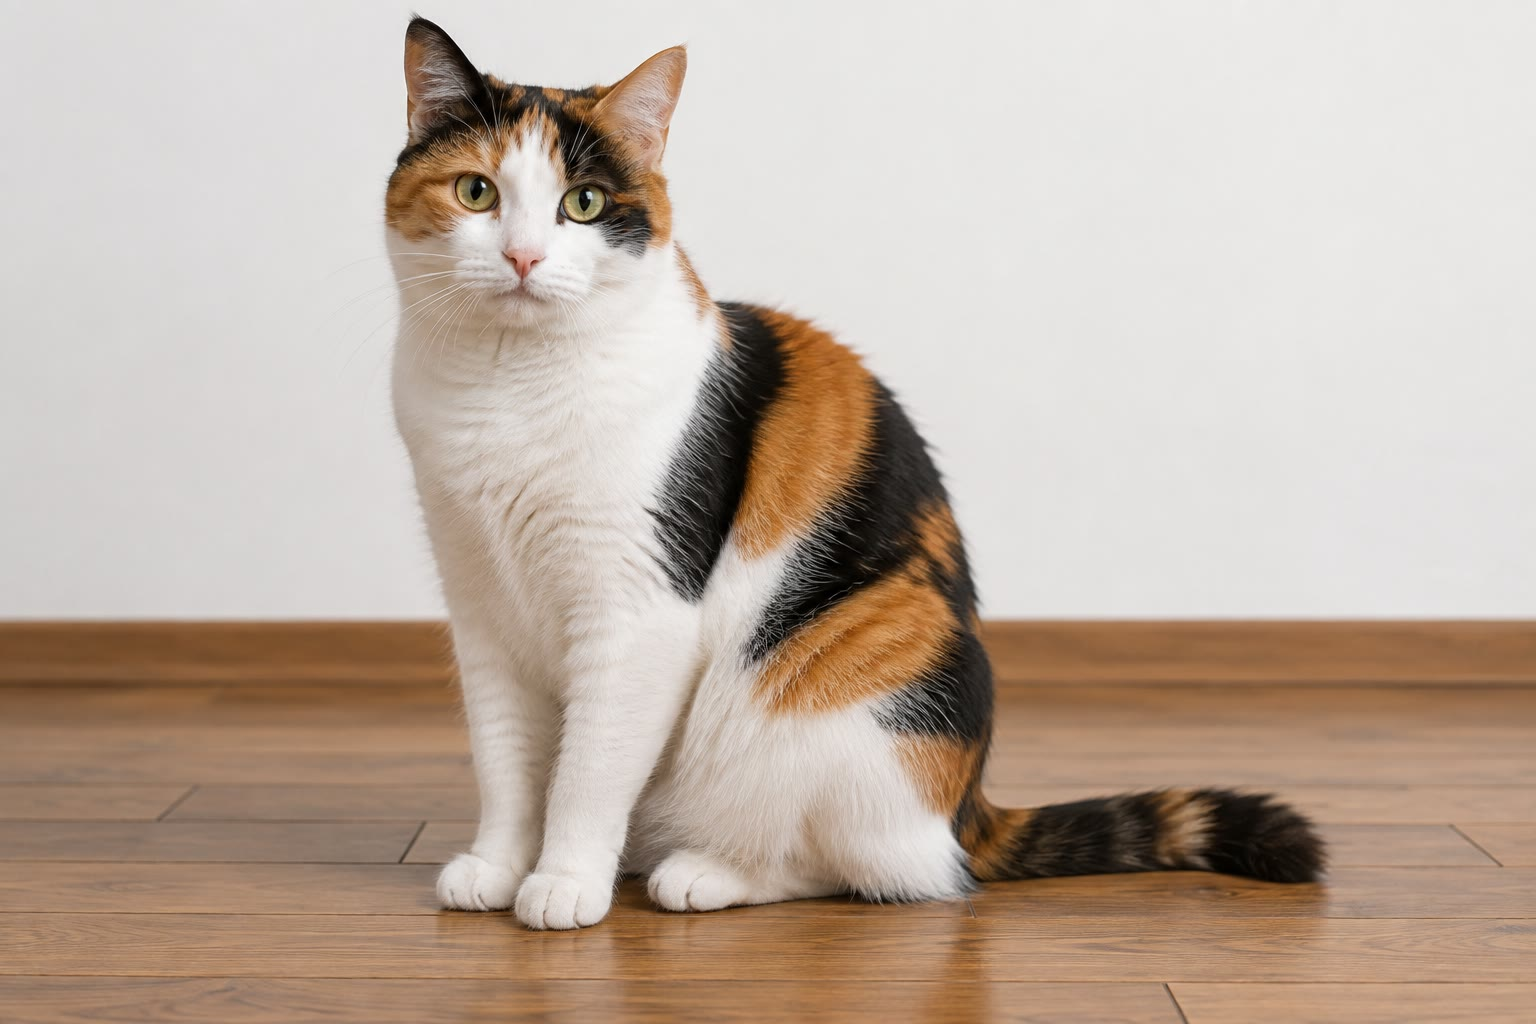
\includegraphics[width=0.5\linewidth]{images/book5/ai/b5-01-calico-cat.jpg}

{\small Izquierda: un núcleo femenino teñido para el ADN, con el X
inactivo compacto --- el \omterm{def:b3:chromatin-epigenetics:x-inactivation}{corpúsculo de Barr} --- apretado contra el borde
nuclear. Derecha: una gata carey. Cada mancha naranja o negra es un clon
de células de la piel que silenciaron el mismo cromosoma X; el blanco se
debe a otro gen distinto, autosómico, de moteado.}
\end{omfigure}

\begin{definition}[Impronta genómica]\label{def:b3:chromatin-epigenetics:imprinting}
\index{impronta genómica}\index{región de control de la impronta}\index{disomía uniparental}
Un gen está \emph{improntado} cuando solo se expresa uno de sus dos
alelos, y cuál de ellos depende del progenitor del que venga: algunos
genes se expresan solo desde la copia paterna y otros solo desde la
materna. Los mamíferos tienen entre \numrange{100}{200} genes
improntados, agrupados, y cada agrupamiento lo gobierna una \emph{región
de control de la impronta} (ICR) que está metilada en uno de los alelos
parentales y no en el otro. La metilación se establece en la línea
germinal --- un patrón en el espermatozoide y otro en el óvulo ---, se
borra en las células germinales de la generación siguiente y se vuelve a
poner según el sexo de ese individuo. Un niño que recibe las dos copias
de un cromosoma del mismo progenitor (\emph{disomía uniparental}) tiene
por tanto una dosis equivocada de los genes improntados que lleva, aunque
su secuencia sea del todo normal.
\end{definition}

\begin{proof}[Evidencia]
McGrath y Solter, e independientemente Surani, Barton y Norris (1984),
hicieron cigotos de ratón con dos pronúcleos maternos, o con dos
paternos, transfiriendo pronúcleos entre huevos fecundados. Ninguno de
los dos tipos llegó a término, aunque cada uno tenía dos juegos completos
de cromosomas: los embriones ginogenéticos formaban un embrión razonable
con una placenta pobre, y los androgenéticos una placenta grande y casi
ningún embrión. Los dos genomas parentales no son equivalentes y ambos
son necesarios. Cattanach y Kirk (1985) demostraron, con \omterm{def:b3:chromatin-epigenetics:imprinting}{disomías
uniparentales} de cromosomas concretos, que la no equivalencia se limita a
regiones concretas de cromosomas concretos, que son donde más tarde se
encontraron los agrupamientos improntados.
\end{proof}

\begin{example}[El agrupamiento \emph{Igf2}--\emph{H19}]\label{ex:b3:chromatin-epigenetics:igf2}
\emph{Igf2}, un factor de crecimiento fetal, se expresa desde el alelo
paterno; su vecino \emph{H19}, un ARN no codificante, desde el materno.
Entre ambos está la ICR y, más allá de \emph{H19}, un conjunto compartido
de potenciadores. En el cromosoma materno la ICR no está metilada y une
CTCF, que actúa como aislante: los potenciadores pueden alcanzar a
\emph{H19} pero no a \emph{Igf2}. En el cromosoma paterno la ICR está
metilada (se fijó en el espermatozoide), CTCF no puede unirse y los
potenciadores alcanzan a \emph{Igf2}; la metilación se extiende además
hasta silenciar el promotor de \emph{H19}. Una sola marca, puesta en una
sola línea germinal, decide los dos genes.
\end{example}

\begin{omfigure}
\begin{tikzpicture}[every node/.style={font=\scriptsize}, >=stealth]
  \foreach \yy/\lab/\ctcf in {1.6/cromosoma materno/1, -0.6/cromosoma paterno/0} {
    \draw[very thick, gray] (0,\yy) -- (9.4,\yy);
    \node[left, align=right] at (-0.15,\yy) {\lab};
    \draw[thick, fill=omDef!25] (1.0,\yy-0.2) rectangle (2.6,\yy+0.2); \node at (1.8,\yy) {\emph{Igf2}};
    \draw[thick, fill=omProp!30] (4.2,\yy-0.2) rectangle (5.2,\yy+0.2); \node at (4.7,\yy) {ICR};
    \draw[thick, fill=omDef!25] (6.2,\yy-0.2) rectangle (7.4,\yy+0.2); \node at (6.8,\yy) {\emph{H19}};
    \foreach \x in {8.4,8.8,9.2} \fill[omMeth!70!black] (\x,\yy) circle (0.12);
    \node[right] at (9.55,\yy) {potenciadores};
  }
  % maternal: CTCF bound, enhancer -> H19
  \draw[thick, fill=omExo!35] (4.7,2.15) ellipse (0.45 and 0.22); \node at (4.7,2.15) {CTCF};
  \draw[->, thick, omMeth!70!black] (8.4,1.85) .. controls (7.8,2.5) and (7.2,2.5) .. (6.8,1.85);
  \node[above] at (7.6,2.35) {activo};
  \draw[thick, omThm] (5.3,2.3) -- (5.3,0.9); \node[omThm, below] at (5.3,0.9) {aislante};
  \node[omThm, above=1.0cm, align=center, font=\scriptsize] at (1.8,1.8) {\emph{Igf2} silencioso};
  % paternal: ICR methylated
  \foreach \x in {4.35,4.6,4.85,5.1} \fill[omThm] (\x,-0.95) circle (0.08);
  \node[below, align=center] at (4.7,-1.05) {metilada:\\sin CTCF};
  \draw[->, thick, omMeth!70!black] (8.4,-0.35) .. controls (6.5,0.6) and (3.5,0.6) .. (1.8,-0.35);
  \node[above] at (3.3,0.2) {activo};
  \foreach \x in {6.4,6.7,7.0,7.2} \fill[omThm] (\x,-0.95) circle (0.08);
  \node[below] at (6.8,-1.05) {silenciado};
\end{tikzpicture}

{\small La impronta en \emph{Igf2}--\emph{H19}. Alelo materno: la ICR sin
metilar une CTCF, un aislante, de modo que los potenciadores de aguas
abajo solo activan \emph{H19}. Alelo paterno: la ICR se metiló en el
espermatozoide, CTCF no puede unirse, los potenciadores alcanzan a
\emph{Igf2} y la metilación silencia \emph{H19}.}
\end{omfigure}

\begin{example}[Prader--Willi y Angelman]\label{ex:b3:chromatin-epigenetics:pws}
La misma deleción de unos \qty{5}{Mb} en el cromosoma 15 (región
15q11--q13) causa el \emph{síndrome de Prader--Willi} --- hipotonía
muscular al nacer y después apetito insaciable y obesidad --- cuando está
en el cromosoma paterno, y el \emph{síndrome de Angelman} ---
discapacidad intelectual grave, ausencia de habla, un porte risueño y
convulsiones --- cuando está en el materno. La región lleva genes de
expresión paterna (\emph{SNRPN} y un agrupamiento de ARN pequeños) cuya
única copia activa se pierde en el primer caso, y el gen de expresión
materna \emph{UBE3A}, que se pierde en el segundo. La \omterm{def:b3:chromatin-epigenetics:imprinting}{disomía uniparental}
materna del 15, sin deleción ninguna, da también un Prader--Willi: dos
copias maternas, silenciosas para los genes paternos.
\end{example}

\begin{remark}[Por qué improntar]\label{rem:b3:chromatin-epigenetics:kinship}
Los genes improntados están enriquecidos en el control del crecimiento
fetal y del transporte de nutrientes por la placenta, y los de expresión
paterna (\emph{Igf2}, \emph{Peg3}) tienden a favorecer el crecimiento
mientras que los de expresión materna (\emph{H19}, \emph{Igf2r},
\emph{Cdkn1c}) tienden a frenarlo. La \emph{teoría del parentesco} lee
esto como un conflicto: los genes de un padre ganan extrayendo más de una
madre que quizá lleve más tarde crías de otros machos, mientras que los
de la madre ganan racionando entre todas sus camadas. La impronta se da
en los mamíferos placentarios y en las plantas con flor, cuyo endospermo
también lo alimenta la madre, y no en las aves ni en los reptiles, que es
lo que predice la teoría.
\end{remark}

\section{La herencia epigenética y sus límites}

\begin{definition}[Epigenética]\label{def:b3:chromatin-epigenetics:epigenetics}
\index{epigenética}\index{epialelo}\index{reprogramación}
La \emph{epigenética} es el estudio de los cambios heredables de la
actividad génica que no son cambios de la secuencia del ADN: estados
llevados por la \omterm{def:b3:chromatin-epigenetics:methylation}{metilación del ADN}, por las marcas de \omterm{def:b3:chromatin-epigenetics:nucleosome}{histonas} o por
circuitos autosostenidos de factores de transcripción, y copiados a
través de la división celular. Dos alelos de secuencia idéntica pero de
estado epigenético estable distinto son \emph{epialelos}. La herencia a
través de la mitosis es la regla y es lo que hace que una célula
diferenciada siga diferenciada. La herencia a través de la meiosis, de
padres a hijos, es la excepción en los mamíferos, porque las marcas se
borran en dos oleadas de \emph{reprogramación}: en las células germinales
primordiales, donde se barren las improntas y casi toda la metilación
para volver a fijarlas según el sexo, y otra vez en el cigoto y el
embrión temprano, donde el genoma paterno se desmetila activamente por
TET3 y el materno de forma pasiva, antes de que DNMT3 establezca los
patrones propios del embrión.
\end{definition}

\begin{example}[El ratón agutí viable amarillo]\label{ex:b3:chromatin-epigenetics:agouti}
En el alelo $A^{vy}$ un retrotransposón se ha insertado aguas arriba del
gen de color del pelaje \emph{agouti}. Donde el promotor del transposón
no está metilado, dirige la expresión constante de \emph{agouti} en todas
las células; el ratón es amarillo, obeso y propenso a la diabetes. Donde
está metilado, el gen sigue su control normal y el ratón es pardo
(``seudoagutí''). Hermanos de camada genéticamente idénticos se reparten
por todo el espectro, y una madre amarilla tiene más crías amarillas que
una parda: el \omterm{def:b3:chromatin-epigenetics:epigenetics}{epialelo} se borra de forma incompleta a través de la línea
germinal materna. Waterland y Jirtle (2003) alimentaron a madres $A^{vy}$
preñadas con una dieta rica en donadores de metilo (folato, vitamina
B\textsubscript{12}, colina, betaína) y desplazaron el pelaje de las
crías hacia el pardo. El ambiente de una generación había fijado una
marca que llevó la siguiente.
\end{example}

\begin{omfigure}
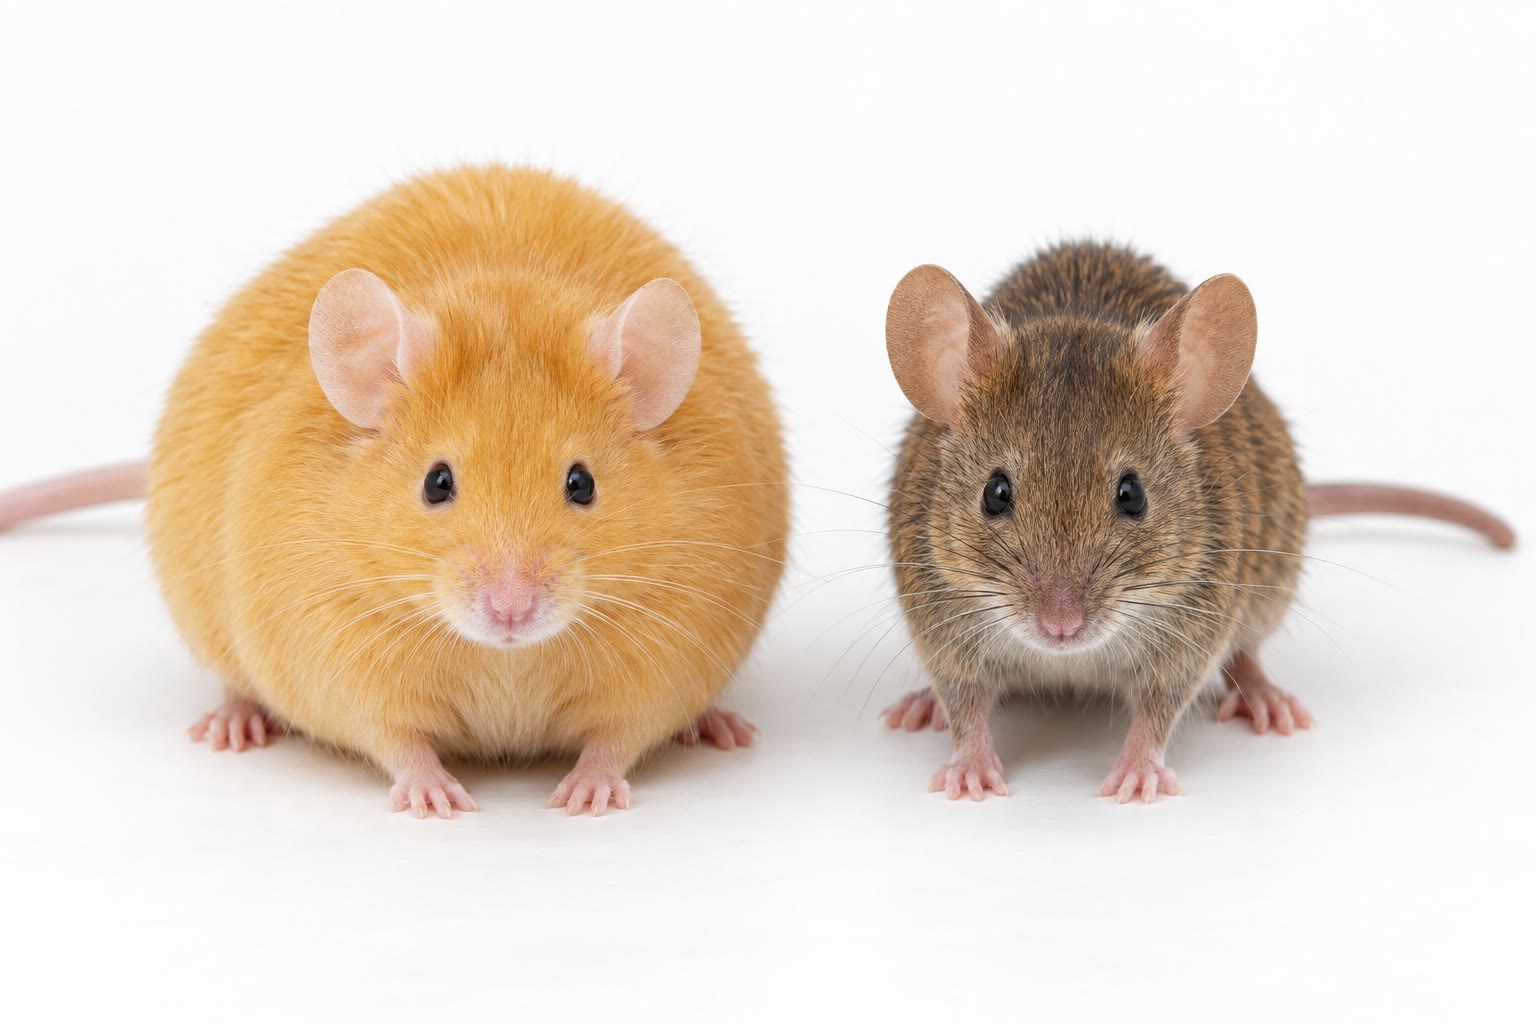
\includegraphics[width=0.62\linewidth]{images/book5/ai/b5-01-agouti-mice.jpg}

{\small Dos hermanos de camada $A^{vy}$ de genotipo idéntico: un ratón
amarillo y obeso en el que el transposón situado aguas arriba de
\emph{agouti} no está metilado y un seudoagutí pardo en el que sí lo está.}
\end{omfigure}

\begin{proposition}[Dónde se encuentran estados epigenéticos heredables]\label{prop:b3:chromatin-epigenetics:examples}
\index{variegación por efecto de posición}\index{vernalización}\index{paramutación}
Tres sistemas bien analizados ilustran los mecanismos anteriores. La
\emph{\omterm{prop:b3:chromatin-epigenetics:examples}{variegación por efecto de posición}} en \emph{Drosophila}: un gen
que una reorganización cromosómica traslada junto a \omterm{def:b3:chromatin-epigenetics:nucleosome}{heterocromatina} queda
silenciado en unas células y no en otras, lo que da un ojo moteado; cada
mancha es un clon, el silenciamiento se propaga desde la \omterm{def:b3:chromatin-epigenetics:nucleosome}{heterocromatina}
por el bucle de HP1, y los genes cuya mutación suprime la variegación
(los genes \emph{Su(var)}) son HP1 y la metiltransferasa de H3K9. La
\emph{vernalización} en \emph{Arabidopsis}: semanas de frío invernal
silencian el represor de la floración \emph{FLC} mediante la H3K27me3
depositada por Polycomb, el silencio aguanta meses de crecimiento
primaveral y miles de divisiones celulares, y se restablece en cada
generación, de modo que cada planta ha de pasar su propio invierno. La
\emph{paramutación} en el maíz: un alelo del gen de pigmentación
\emph{b1}, cuando se encuentra con otro alelo determinado en un
heterocigoto, lo convierte a su propio estado silencioso, y el alelo
convertido transmite el estado a sus descendientes durante generaciones,
mediante una metilación dirigida por ARN pequeños que se retoma en
\cref{ch:b3:rna-regulation}. En cada caso la herencia es mitótica y
robusta; la transmisión entre generaciones o bien se restablece
activamente (plantas) o bien es parcial y con fugas (ratones).
\end{proposition}

\begin{remark}[Los límites de las afirmaciones transgeneracionales]\label{rem:b3:chromatin-epigenetics:limits}
Las afirmaciones de que los nietos humanos heredan ``epigenéticamente''
la hambruna o el estrés de un abuelo son frecuentes y en su mayor parte
no están demostradas. Entre una marca somática y un nieto median dos
oleadas de borrado; los genes improntados y unos pocos transposones son
los únicos supervivientes documentados del borrado en los mamíferos; y en
las cohortes humanas los efectos de un ambiente compartido, del ambiente
uterino y de las diferencias genéticas son difíciles de separar de una
marca llevada en la línea germinal. Los casos demostrados --- el $A^{vy}$,
algunos \omterm{def:b3:chromatin-epigenetics:epigenetics}{epialelos} ligados a transposones, los estados mediados por ARN en
gusanos y plantas --- son reales, están entendidos molecularmente y son
estrechos. El teorema del capítulo dice por qué: sin una retroalimentación
que empuje $\mu$ hacia $1$, una marca se olvida a sí misma en unas pocas
docenas de divisiones, y la línea germinal añade encima un borrado activo.
\end{remark}

\section{Ejercicios}

\begin{exercise}[$\star$]\label{exo:b3:chromatin-epigenetics:1}
Dese la composición de una partícula nuclear de \omterm{def:b3:chromatin-epigenetics:nucleosome}{nucleosoma}, la longitud
de ADN que une y la longitud típica del enlazador. ¿Por qué la digestión
de la \omterm{def:b3:chromatin-epigenetics:nucleosome}{cromatina} con nucleasa dio una escalera de fragmentos y no una
mancha continua?
\end{exercise}

\begin{exercise}[$\star$]\label{exo:b3:chromatin-epigenetics:2}
Un genoma de rana tiene $3.0\times 10^{9}$ pares de bases por juego
haploide. ¿Cuántos \omterm{def:b3:chromatin-epigenetics:nucleosome}{nucleosomas} contiene un núcleo diploide, tomando una
repetición de \qty{190}{bp}, y qué longitud tiene su ADN?
\end{exercise}

\begin{exercise}[$\star$]\label{exo:b3:chromatin-epigenetics:3}
Descífrense H3K27me3, H4K16ac y H3S10ph. Dígase para cada una si se
asocia a \omterm{def:b3:chromatin-epigenetics:nucleosome}{cromatina} activa o silenciosa, y nómbrese un \omterm{def:b3:chromatin-epigenetics:histone-code}{lector} de la
primera.
\end{exercise}

\begin{exercise}[$\star$]\label{exo:b3:chromatin-epigenetics:4}
Explíquese por qué una gata carey es casi siempre hembra, y qué tiene que
ser un carey macho.
\end{exercise}

\begin{exercise}[$\star\star$]\label{exo:b3:chromatin-epigenetics:5}
Calcúlese la \omterm{prop:b3:chromatin-epigenetics:compaction}{razón de empaquetamiento} de la fibra de \qty{10}{nm} a
partir de los números de
\cref{def:b3:chromatin-epigenetics:nucleosome} (repetición \qty{200}{bp},
cuenta \qty{11}{nm}), y la razón necesaria para meter los \qty{4}{cm} de
ADN de un cromosoma humano medio en una cromátida mitótica de
\qty{4}{\micro m}. ¿Por qué factor adicional debe plegarse la fibra?
\end{exercise}

\begin{exercise}[$\star\star$]\label{exo:b3:chromatin-epigenetics:6}
En el modelo de \cref{thm:b3:chromatin-epigenetics:maintenance} con
$\mu = 0.98$ y $\delta = 0.01$, hállense $p^{*}$ y el número de
divisiones tras las cuales un sitio que empezó metilado ha perdido la
mitad de su exceso sobre $p^{*}$. Repítase para $\mu = 0.999$,
$\delta = 0.001$.
\end{exercise}

\begin{exercise}[$\star\star$]\label{exo:b3:chromatin-epigenetics:7}
Un experimento de ChIP-seq en células de hígado da un pico de H3K4me3 y
un pico de H3K27ac en el promotor del gen $A$, un dominio ancho de
H3K27me3 sobre el gen $B$ y H3K9me3 sobre el gen $C$. Predígase el estado
transcripcional de cada uno, y dígase cuál de $B$ y $C$ tiene más
probabilidades de encenderse en otro tipo celular, y por qué.
\end{exercise}

\begin{exercise}[$\star\star$]\label{exo:b3:chromatin-epigenetics:8}
Una mujer lleva una deleción de la región de \emph{UBE3A} en uno de sus
cromosomas 15 pero está sana. Su padre llevaba la misma deleción y
también estaba sano. ¿Qué síndrome, si alguno, corre el riesgo de tener
cada uno de sus hijos, y con qué probabilidad? ¿Y si la deleción le
hubiera venido de su madre?
\end{exercise}

\begin{exercise}[$\star\star$]\label{exo:b3:chromatin-epigenetics:9}
Predígase la consecuencia, en un embrión de ratón hembra, de suprimir el
gen \emph{\omterm{def:b3:chromatin-epigenetics:x-inactivation}{Xist}} de uno de los cromosomas X; y de los dos. Predígase qué
le hace a un autosoma un transgén de \emph{\omterm{def:b3:chromatin-epigenetics:x-inactivation}{Xist}} insertado en él.
\end{exercise}

\begin{exercise}[$\star\star\star$]\label{exo:b3:chromatin-epigenetics:10}
Explíquese, con \cref{ex:b3:chromatin-epigenetics:cpg-deficit}, por qué
las \omterm{def:b3:chromatin-epigenetics:methylation}{islas CpG} han conservado sus \omterm{def:b3:chromatin-epigenetics:methylation}{CpG} mientras que el resto del genoma ha
perdido cuatro quintas partes de los suyos, y qué implica esto sobre el
estado de metilación de las islas en la línea germinal a lo largo del
tiempo evolutivo. ¿Por qué falla el argumento para un gen metilado solo
en el hígado?
\end{exercise}

\begin{exercise}[$\star\star\star$]\label{exo:b3:chromatin-epigenetics:11}
Muéstrese, con el bucle escritor--lector de
\cref{prop:b3:chromatin-epigenetics:readers}, cómo un dominio de H3K9me3
puede ser estable a través de la replicación aunque cada división diluya
al doble las \omterm{def:b3:chromatin-epigenetics:nucleosome}{histonas} marcadas con otras nuevas sin marcar. ¿Qué
determina dónde deja de propagarse el dominio? Propóngase un experimento
que ponga a prueba la explicación.
\end{exercise}

\begin{exercise}[$\star\star\star$]\label{exo:b3:chromatin-epigenetics:12}
Un estudio informa de que los nietos de personas que pasaron una hambruna
tienen alterada la metilación de un gen del crecimiento y una masa
corporal mayor. Enumérense las explicaciones alternativas que hay que
excluir antes de concluir que se transmitió una marca de metilación por
la línea germinal, y dígase qué experimento en ratones zanjaría la
cuestión.
\end{exercise}

\section{Problema: la memoria de un gen silenciado}

\begin{problem}[{Problema de fin de semana --- un genoma humano
empaquetado en su núcleo, una marca de metilación seguida a lo largo de
las divisiones, una gata carey leída como un mapa clonal y las
enfermedades de una región improntada contadas, hasta llegar al número de
divisiones que sobrevive una marca sin retroalimentación y al tamaño de
la población celular que eligió su X}]
\label{pb:b3:chromatin-epigenetics:1}
Datos: un núcleo humano diploide contiene $6.4\times 10^{9}$ pares de
bases, a \qty{0.34}{nm} y \qty{650}{Da} por par; la repetición del
\omterm{def:b3:chromatin-epigenetics:nucleosome}{nucleosoma} es de \qty{200}{bp}, un octámero de \omterm{def:b3:chromatin-epigenetics:nucleosome}{histonas} pesa
\qty{108}{kDa} y una partícula nuclear es un disco de \qty{11}{nm} de
diámetro y \qty{5.5}{nm} de espesor. El núcleo es una esfera de
\qty{10}{\micro m} de diámetro. El genoma tiene un \qty{42}{\%} de
G$+$C. Metilación en un \omterm{def:b3:chromatin-epigenetics:methylation}{CpG} corriente: $\mu = 0.99$, $\delta = 0.02$ por
división.

\medskip
\noindent\textbf{Parte I --- Empaquetamiento.}
\begin{enumerate}
  \item Calcúlense la longitud total del ADN del núcleo y el número de
        \omterm{def:b3:chromatin-epigenetics:nucleosome}{nucleosomas}.
  \item Calcúlense la masa total de \omterm{def:b3:chromatin-epigenetics:nucleosome}{histona} (solo octámeros) y la de
        ADN, en picogramos ($\qty{1}{Da} = \qty{1.66e-24}{g}$).
  \item Calcúlense el volumen del núcleo y el volumen total de las
        partículas nucleares, tratadas como cilindros. ¿Qué fracción del
        núcleo llenan?
  \item Si los \omterm{def:b3:chromatin-epigenetics:nucleosome}{nucleosomas} se pusieran uno tras otro como una fibra de
        \qty{10}{nm}, ¿qué longitud tendría la fibra y cuál es la \omterm{prop:b3:chromatin-epigenetics:compaction}{razón
        de empaquetamiento} respecto al ADN desnudo?
  \item La fibra se pliega en bucles de \qty{200}{kb} anclados por
        cohesina. ¿Cuántos bucles, y cuántos \omterm{def:b3:chromatin-epigenetics:nucleosome}{nucleosomas} por bucle?
  \item Bajo la hipótesis de independencia, ¿cuántos dinucleótidos \omterm{def:b3:chromatin-epigenetics:methylation}{CpG}
        contendría el genoma diploide? El número observado es
        $5.6\times 10^{7}$. ¿Qué fracción se ha perdido, y por qué
        mecanismo mutacional?
\end{enumerate}

\medskip
\noindent\textbf{Parte II --- Una marca a lo largo de las divisiones.}
\begin{enumerate}[resume]
  \item Escríbase la recurrencia de $p_{n}$ y calcúlese $p^{*}$.
  \item Un \omterm{def:b3:chromatin-epigenetics:methylation}{CpG} de promotor está completamente metilado en $n = 0$.
        Calcúlese $p_{n}$ tras $10$, $50$ y $200$ divisiones.
  \item ¿Al cabo de cuántas divisiones se ha reducido a la mitad el
        exceso $p_{n} - p^{*}$? Una célula madre de un tejido se divide
        una vez por semana: ¿cuántos años son?
  \item Un fármaco inhibe por completo la \omterm{def:b3:chromatin-epigenetics:methylation}{DNMT1} ($\mu = 0$) y también la
        DNMT3 ($\delta = 0$). Muéstrese que la fracción de hebras
        metiladas de la población se reduce a la mitad en cada división,
        y hállese el número de divisiones para bajar de un
        \qty{80}{\%} de metilación a menos de un \qty{5}{\%}.
  \item En una isla silenciada los \omterm{def:b3:chromatin-epigenetics:histone-code}{lectores} de \omterm{def:b3:chromatin-epigenetics:methylation}{CpG} metilado reclutan
        metilación de H3K9, que recluta a DNMT3, de modo que dentro de la
        isla $\mu = 0.9995$ y $\delta = 0.0005$. Recalcúlese la
        semivida del exceso, en divisiones y en años a una división por
        semana.
  \item Explíquese en una frase por qué lo que necesita un gen silenciado
        de por vida es el resultado de la pregunta 11 y no el de la 9, y
        qué clase de disposición molecular lo produce.
\end{enumerate}

\medskip
\noindent\textbf{Parte III --- El mapa de la gata carey.}
\begin{enumerate}[resume]
  \item Una gata es heterocigótica para el gen naranja ligado al X.
        Explíquese por qué su pelaje tiene manchas naranjas y negras y
        qué representa una mancha.
  \item La \omterm{def:b3:chromatin-epigenetics:x-inactivation}{inactivación del X} ocurrió cuando las células destinadas a
        formar la piel eran $N$. Cada una eligió un X al azar. ¿Cuál es
        la probabilidad de que las $N$ eligieran el mismo, dando una gata
        de un solo color?
  \item No se ha documentado ninguna heterocigótica de un solo color
        entre quizá mil millones de gatos; tómese la probabilidad como
        $10^{-9}$ y estímese $N$.
  \item La superficie de la piel de la gata es de unos \qty{0.3}{m^2} y
        sus manchas miden en promedio \qty{15}{cm^2}. Estímese el número
        de manchas y explíquese por qué es mayor que $N$.
  \item Un gato XXY es también carey. ¿Cuántos \omterm{def:b3:chromatin-epigenetics:x-inactivation}{corpúsculos de Barr}
        muestran sus células? ¿Cuántos en una hembra XXX y en un macho
        XY?
  \item Un gen que escapa a la inactivación está presente en dos copias
        activas en las hembras y en una en los machos. Dese una razón por
        la que ese escape puede tolerarse y una situación en la que
        importe.
\end{enumerate}

\medskip
\noindent\textbf{Parte IV --- El cromosoma 15.}
\begin{enumerate}[resume]
  \item El síndrome de Prader--Willi afecta a uno de cada
        \num{15000} nacimientos; el \qty{70}{\%} de los casos son una
        deleción de novo del 15q11--q13 paterno y el \qty{25}{\%} una
        \omterm{def:b3:chromatin-epigenetics:imprinting}{disomía uniparental} materna. Calcúlese la frecuencia de
        nacimiento de cada causa.
  \item El síndrome de Angelman tiene aproximadamente la misma
        frecuencia; el \qty{70}{\%} son deleciones maternas, el
        \qty{5}{\%} disomías paternas y el \qty{10}{\%} mutaciones
        puntuales de \emph{UBE3A}. ¿Por qué las mutaciones puntuales son
        causa de Angelman y casi nunca de Prader--Willi?
  \item Un padre lleva una translocación equilibrada que da al
        \qty{20}{\%} de sus espermatozoides una deleción de 15q11--q13.
        ¿Qué fracción de sus hijos tiene Prader--Willi y qué fracción
        Angelman?
  \item La \omterm{def:b3:chromatin-epigenetics:imprinting}{disomía uniparental} surge cuando un cigoto trisómico pierde un
        cromosoma. Si un cigoto con trisomía 15 pierde al azar uno de sus
        tres cromosomas, y la trisomía venía de la madre (dos copias
        maternas), ¿cuál es la probabilidad de que el superviviente tenga
        disomía materna? ¿Qué síndrome?
  \item Los genes de Prader--Willi son de expresión paterna y el de
        Angelman, de expresión materna. Usando la teoría del parentesco,
        dígase cuáles de los síntomas de los dos síndromes (dificultad
        para mamar al nacer frente a apetito voraz) encajan en la teoría
        y cuáles son más difíciles de encajar.
  \item Se propone un método para tratar el Angelman reactivando el
        \emph{UBE3A} paterno silencioso. Su silencio se debe a un ARN
        antisentido de expresión paterna. Propóngase la diana molecular y
        dígase por qué la terapia no perturbaría a los demás genes
        improntados.
  \item Resúmase: la semivida de una marca sin retroalimentación
        (pregunta~9) y con ella (pregunta~11), en divisiones; y la
        población fundadora $N$ del pelaje de la gata carey
        (pregunta~15).
\end{enumerate}
\end{problem}
